\section{Proposed approach} \label{s:methods}

\subsection{Datasets} \label{sec:datapreparation}
The datasets used in this study are MIMIC II (Physionet MIMICII) \cite{MIMIC2} and MIMIC III (Physionet-MIMICIII) \cite{MIMIC3}. These databases are developed by the Multi-parameter Intelligent Monitoring in Intensive Care (MIMIC) project at the Laboratory of Computational Physiology at MIT, funded by the National Institute of Biomedical Imaging and Bioengineering. For each dataset the data holds the results of lab tests produced through each test done on each patient. Each lab test result contains the numeric value of the lab test performed, a flag (binary) indicating whether the result is ``normal'' or ``abnormal'', the unit of measurement, and date/time of the test performed. 

\subsubsection{MIMIC II} \label{sec:MIMIC2}
MIMIC II data were collected between 2001 and 2008 from a variety of ICUs. MIMIC II database contains the records of 33,000 patients of which around 25,000 are adults (having age $\geq$ 15 years at time of last admission) and near about 8000 are neonates (age $\leq$ 1 month at the time of first admission). These patients were admitted into over 36,000 hospitals and stayed in over 40,000 ICUs. MIMIC II consists of two major components: clinical data and physiological waveforms. The clinical data are used in this study.   

This clinical dataset consists 40 different tables, each containing different types of information, such  as, demographic data (available in \textit{General} category), hospital admission data, ICU stay data, medication information, lab test results (available in \textit{Labtests}), nurse notes and so on. Among these tables, only the lab test data is used in this work to investigate the effectiveness thereof in predicting mortality. In addition to the lab test results, the patient's final status, i.e., whether the patient survived or died in the ICU is used. 

\subsubsection{MIMIC III} \label{sec:MIMIC3}
MIMIC III data were collected between 2001 to 2012 from more than 50,000 hospital admissions. This database comprises 25 different tables, each holding different types of information, for example, demographic data, hospital admission data, ICU stay data, medication information, lab test results, nurse notes and so on. The lab test data (called \textit{Labevents}) as well as some demographic and admission related information from among these tables are used primarily in our study.

The \textit{Patient} table, which contains the date of birth, gender, and whether the patient survived or died is used in this work. The \textit{Admissions} table, which holds the date of admission, date of discharge, ethnicity, and diagnosis of the patient is also used here. The patient's age is computed by joining the \textit{Patient} table and \textit{Admissions} table and they by deducting the date of birth from the date of admission. Finally, the \textit{ICUStays} table, that contains the length of stay of the patient, is used in this study.

\subsubsection{Feature extraction and vector generation} 
\textcolor{blue}{At first, we make a profile for each patient based on his/her age as has been done in \cite{mehedy-masud:2017:fvc} and form four different groups: Newborn, Infant, Child, Adult, and Senior. Table \ref{t:groupbyage} shows the information of the age for these groups. In line with the work of \cite{mehedy-masud:2017:fvc, mehedy-masud:2018:frmwrk}, we also consider \textit{Adult} and \textit{Senior} groups only.}

\begin{table}[h] 
	\centering \caption{\textcolor{blue}{Information of the age of the groups}} 
	\begin{tabular}{|l||l|}\hline
		\textbf{Group}  & \textbf{Age}  \\\hline
		Newborn & 0-3M \\\hline
		Infant &  4M-2Y\\\hline
		Child & 3Y-17Y \\\hline
		Adult & 18Y-64Y \\\hline
		Senior & 65Y+ \\\hline
	\end{tabular}
	\label{t:groupbyage}
\end{table} 

Features are extracted from the \textit{Labtests} table for MIMIC II and the \textit{Labevents} table from MIMIC III as follows. First, a list of all different lab tests done on the selected patients are enumerated. This is denoted as the feature set. Then for each patient, the test results are extracted for each feature from the records of that patient. This needs searching through several millions of lab test records. If a particular test was not performed and monitored on the patient, then the corresponding feature value is regarded as missing, and if the test was administered more than once, the average (last) is taken for MIMIC II (MIMIC III) dataset. Notably, for MIMIC III dataset, a more appropriate treatment in this case (i.e., more than one values) can be performed by adapting a longitudinal feature treatment approach; this is left as a future work. Table \ref{t:datasetoverview} shows an overview of the datasets used in this study. Note that we have randomly partitioned the datasets into training \& testing samples.

\begin{table}[h] 
	\centering \caption{Overview on the datasets} 
	\begin{tabular}{|l||l||l||l||l||l|}\hline
			\textbf{MIMIC Type} & 	\textbf{Age Type} & \textbf{Data Type}  & \textbf{No. of Training Samples} & \textbf{No. of Testing Samples} & \textbf{No. of Features} \\\hline
			II & Adult & Binary(F) & 3352 & 1481 & 656 \\\hline
			II & Adult & Numeric(V) & 3352 & 1481 & 656 \\\hline
			II & Senior & Binary(F) & 3614 & 1996 & 557 \\\hline
			II & Senior & Numeric(V) & 3614 & 1996 & 557 \\\hline
			III & Adult & Numeric(V) & 3352 & 1481 & 657 \\\hline
			III & Senior & Numeric(V) & 3614 & 1996 & 558 \\\hline
	\end{tabular}
	\label{t:datasetoverview}
\end{table} 
  
 
\subsection{Model Construction Overview}

\begin{figure}[h]
\centering
\fbox{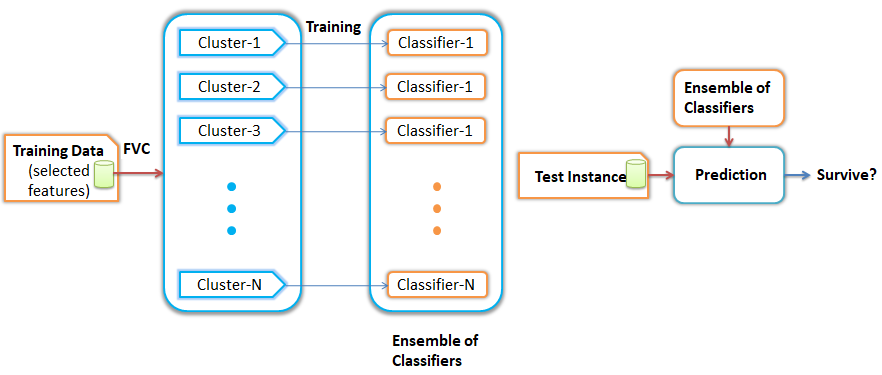
\includegraphics[scale=0.7]{fig/ModelConstructionOverview.png}}
\caption{Model construction overview} \label{fig:ClassificationModelGenerationPhase}
\end{figure}

Figure \ref{fig:ClassificationModelGenerationPhase} presents the high level overview of our model construction methodology. For each dataset, all features are evaluated to understand their importances in the classification task. Several feature ranking algorithms (more details of  these algorithms are in Section \ref{s:feature_ranking_selection}) are applied in this context. Then, based on the ranking scores, a subset of the top-ranked features are selected. Subsequently, training data is clustered using some feature vector compaction (FVC) techniques. Later several classification algorithms are trained on these clusters to form ensemble classifiers.  

\subsection{Feature Ranking and Selection} \label{s:feature_ranking_selection}
\textcolor{blue}{Feature ranking and selection has been successfully applied as an integral step in many machine learning pipeline (recent examples include but not limited to \cite{Zahangir2019, Saifur20181st, Saifur20182nd, Saifur2019})}. Features are evaluated and scored using some ranking algorithms. These evaluators evaluate/rank each of the features in the dataset in the context of the output variable (i.e., the \textit{Class}). Many algorithms are found for ranking features in the literature \cite{Dash:1997, Roberto:2003, Jasmina:2011, Kamkar2015, Baalachandran2015, Zhang2017, Zahangir2019}. \textcolor{blue}{Interestingly some feature ranking algorithms from the Waikato Environment for Knowledge Analysis (popularly known as \textit{Weka}) tool have been found to be useful for medical datasets in \cite{Zahangir2019}. Inspired by \cite{Zahangir2019} we have also used these feature ranking algorithms from \textit{Weka} along with other options.} These are: \textit{InfoGainAttributeEval}, \textit{CorrelationAttributeEval}, \textit{ClassifierAttributeEval} with Random Forest, \textit{ClassifierAttributeEval} with Support Vector Machine (SVM). Once the ranked features are identified, several combinations of features are selected from the feature sets based on the ranking.

\subsection{Feature Vector Compaction}

\begin{figure}[h] 
	\centering 
	\fbox{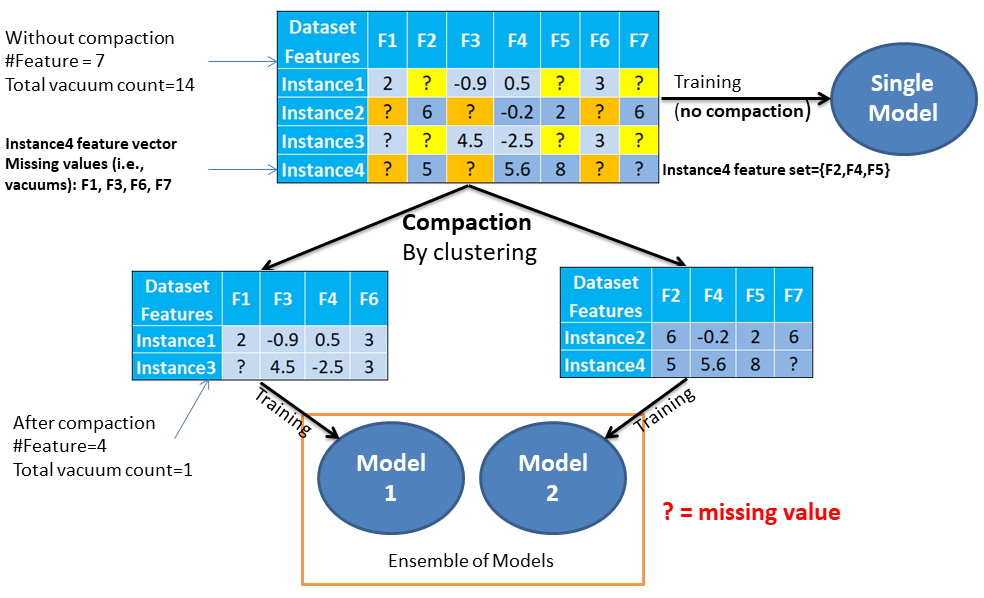
\includegraphics[scale=0.6]{fig/fvc-example-fig.png}}
	\caption{Illustration of Feature Vector Compaction (FVC) technique with example}
	\label{F:fvcwithexample}
\end{figure}

Most of the popular machine learning techniques such as decision tree, SVM and so on, require the feature vector of same features for all instances in order to build predication models. Therefore, for the patient dataset, we need to generate feature vector for each patient by doing the union of the feature sets of all the patients. As a result, empty values are generated for some of the features for some of the patients in the dataset. This sparsity of features not only produces high computational overhead for learning techniques, but also brings noise or redundancy in the data. This issue is increased when we have to work with Big Data, holding thousands of patients information. To deal with the variable feature set we employ Feature Vector Compaction (FVC). It not only minimizes the sparsity of feature vector, but also achieves speedup in learning the prediction and improves the prediction accuracy in most cases. FVC was originally proposed in \cite{mehedy-masud:2017:fvc} by a subset of the authors of this work where some preliminary results were reported. We here exploit FVC and extend its use along several dimensions as will be clear shortly. In general, in FVC technique the patients are grouped (i.e., clustered) according to the similarity of their lab test sets (i.e., feature sets). Figure \ref{F:fvcwithexample} shows the technique with examples.

We also exploit orthogonal clustering (ORCU) which was introduced in \cite{mehedy-masud:2018:frmwrk} by a subset of the authors. Notably, we apply ORCU with some modifications in our research. In orthogonal clustering, dataset is divided into groups in two stages. Every stage has its own clustering technique for grouping data. In the first stage, the dataset is divided by clustering the features (referred to as \textit{Vertical} clustering) and in the second stage, the clustered data from the first stage are further grouped by clustering the subjects (called \textit{Horizontal} clustering).

\begin{algorithm} 
	\caption{ORCU-VH Clustering and Training} 
	\label{a:ORCU-VH}
	{%\footnotesize
		\begin{algorithmic}[1]  
			\REQUIRE {$T$: Raw Training Data}
			\ENSURE { Groups of data $\{D_1, ... D_m\}$ such that 
				$\cup_{i=1}^{m} (D_i) = T$ \\
				$E$: the ensemble classifier,  $E=\{E_1, ... E_m\}$} 
			\STATE $S \leftarrow T$ 
			\STATE $D \leftarrow \phi$
			
			\STATE $S[1], S[2] \leftarrow$ VerticalClustering($S$)//split data using \textit{Vertical} clustering of ORCU					
			
			\FOR {$i \leftarrow$ 1 to 2}
			\STATE $S[i][1], S[i][2] \leftarrow$ HorizontalClustering ($S[i]$) //split data using \textit{Horizontal} clustering of ORCU
			\STATE $D \leftarrow D \cup S[i]$ //generated clusters are put in list
			\ENDFOR
			
			\STATE $m \leftarrow |D|$ //number of data groups
			\FOR {$i \leftarrow$ 1 to $m$}
			\STATE	$E_i \leftarrow $ TrainClassifier($D_i$)
			\ENDFOR    		
		\end{algorithmic}  
	} 
\end{algorithm} 


\begin{algorithm} 
	\caption{ORCU-HV Clustering and Training} 
	\label{a:ORCU-HV}
	{%\footnotesize
		\begin{algorithmic}[1]  
			\REQUIRE {$T$: Raw Training Data}
			\ENSURE { Groups of data $\{D_1, ... D_m\}$ such that 
				$\cup_{i=1}^{m} (D_i) = T$ \\
				$E$: the ensemble classifier,  $E=\{E_1, ... E_m\}$} 
			\STATE $S \leftarrow T$ 
			\STATE $D \leftarrow \phi$
			
			\STATE $S[1], S[2] \leftarrow$ HorizontalClustering($S$)//split data using \textit{Horizontal} clustering of ORCU					
			
			\FOR {$i \leftarrow$ 1 to 2}
			\STATE $S[i][1], S[i][2] \leftarrow$ VerticalClustering($S[i]$) //split data using \textit{Vertical} clustering of ORCU
			\STATE $D \leftarrow D \cup S[i]$ //generated clusters are put in list
			\ENDFOR
			
			\STATE $m \leftarrow |D|$ //number of data groups
			\FOR {$i \leftarrow$ 1 to $m$}
			\STATE	$E_i \leftarrow $ TrainClassifier($D_i$)
			\ENDFOR    		
		\end{algorithmic}  
	} 
\end{algorithm} 

We employ two variations of orthogonal clustering as follows: a) ORCU-VH: in this type, the data is first clustered into two groups by \textit{Vertical} clustering and then the clustered two groups are further divided into four groups using \textit{Horizontal} clustering (please see Algorithm \ref{a:ORCU-VH}); b) ORCU - HV: in this type, the data is clustered in reverse direction of ORCU-VH (i.e., first \textit{Horizontal} clustering followed by \textit{Vertical} clustering) (please see Algorithm \ref{a:ORCU-HV}). 

\subsection{Ensemble Classifiers}
Classifiers are trained on each of the clusters produced at the end of the previous phase. These are used as an ensemble of models $E = {E_1, ...,E_m}$ to classify new patients to predict his mortality. Algorithm 3 (Classify) does the ensemble classification. The input to the algorithm is the instance to be classified, the ensemble of classifiers, and the ensemble approach which is either Vacuum Count (VC) or Common Feature Count (CFC). At first, the test instance is classified by each classifier in the group (the for loop in lines 1-9 does this computation). During this classification process it counts Added Vacuum Count (AVC) \cite{mehedy-masud:2017:fvc} (to be described shortly) or CFC (line 4 and 7). If VC is used then a weighted majority voting is done for the final prediction (lines 10-17). The weight of each model is inversely proportional to the AVC of the test instance and the corresponding dataset of the model. So, lower AVC has higher weight and vice versa. But if CFC is used then the highest CFC value producer (classifier) finally predicts the test instance.  

%But if CFC is used then the prediction of the highest CFC generated ensemble of classifiers is the final prediction (lines 18-21 shows this calculation).       

\begin{algorithm} 
	\caption{Classify} 
	\label{a:Classify}
	{%\footnotesize
		\begin{algorithmic}[1]  
			\REQUIRE {$x$: Instance to classify, $E = \{E_1, ... , E_m \}$: Ensemble of classifiers, $ET = VC$ or $CFC$: Ensemble Technique}
			\ENSURE { $y$: The predicted class} 
			\FOR {$i \leftarrow$ 1 to $m$}
			\STATE $y_i \leftarrow $ Classify($x, E_i$) //Classify
			\IF {$ET = VC$} 	
			\STATE $u_i \leftarrow $ AVC($x, E_i$) //Equation 
			\ref{AVCEquation}
			\ENDIF		
			\IF {$ET = CFC$} 	
			\STATE $u_i \leftarrow $ CFC($x, E_i$) //Equation \ref{CFCEquation}
			\ENDIF		
			\ENDFOR       
			\IF {$ET = VC$}
			\STATE $U \leftarrow \min_{i=1}^m{u_i}$ 
			\FOR {$i \leftarrow$ 1 to $m$}
			\STATE $w_i = U/u_i$       		
			\ENDFOR
			\STATE $W \leftarrow \sum_{i=1}^m{w_i}$ 
			\STATE $y \leftarrow \sum_{i=1}^m{w_i y_i}/W $  			
			\ELSE
			\STATE $i \leftarrow \max_{i=1}^m{u_i}$
			\STATE $y \leftarrow y_i $  
			\ENDIF       
			 
		\end{algorithmic}  
	} 
\end{algorithm} 

\subsubsection{Vacuum counting (VC) method} \label{sec:VCMethod}
Vacuum Count (VC) is the number of vacuums (i.e., empty/missing values) in the instance feature vector. For example, in Figure \ref{F:fvcwithexample}, VC is 4 for \textit{Instance4} (i.e., features F1, F3, F6, and F7 don’t have any value). When two sets of features are merged, the new feature set is created by the union of the two feature sets, which results in generating some vacuums therein. The number of such vacuums is termed as Added vacuums (AVC). For example, suppose a dataset $D$ has feature set $F_D$. If a new instance $d$ is added to $D$, having feature set $F_d$, then the new feature set after merging, $F_{Dnew}$ = $F_D \cup F_d$. Extra vacuums created in the feature vector of $d$ are $|F_{Dnew}|- |F_d|$. So extra vacuums generated in the dataset $D$ are ($|F_{Dnew}| - |F_d|) * n $, where $n$ is the number of instances in $D$ before merging. Therefore, total added vacuums

\begin{equation} \label{AVCEquation}
AVC(D, d) = (|F_{Dnew}| - |F_d|) * (n + 1)
\end{equation}

When an instance of a new patient is considered by the ensemble classification process for prediction, it's missing values are counted with respect to the feature set of each classifier in the ensemble and AVC is computed. 

\subsubsection{Common Feature Counting (CFC) method} \label{sec:CFCMethod}
We propose a new concept called Common Feature Count (CFC) to be used in the ensemble classification process. CFC is defined as follows:

\begin{equation} \label{CFCEquation}
CFC(X,Y_i) = |X \cap Y_i|
\end{equation}

Here, $X$ is the feature set of the corresponding dataset, and $Y_i$ is the (nonempty) feature set of a particular vector $V_i$. For example, if $X$ = {$f_1, f_2, f_3, f_4, f_5$} and $Y_i$ = {$f_2, f_3, f_5, f_6$} then $|X \cap Y_i|$ is 3.

As mentioned earlier, each classifier in the ensemble as well as a test instance has different feature vector. CFC is used to compute the number of common features between a test instance and a classifier in the ensemble. A classification model that has the maximum CFC value is finally used for prediction of this new instance.

%In this methodology, when an instance of new patient is considered into ensemble classification process for prediction, it's CFC is calculated with each cluster for which ensemble model is present. An ensemble model that generates the maximum CFC value is finally used for predicting this new instance.    

%\subsection{Final Model Construction}
%For each dataset, multiple ensemble models are created. In particular, for each dataset, generally 4 separate subset of high ranked features produced by 4 different feature ranking algorithms and four combinations of feature vector grouping, HV, H, VH, V. Thus it leads to form many ensemble models with different combination. We refer to these models using the following form: Model$_{<i>}^{<datasetID-combination>}, 1\leq i \leq 800$. Figure \ref{F:ModelGenOverview} shows how 800 models are generated.

%\begin{figure}[h] 
%	\centering 
%	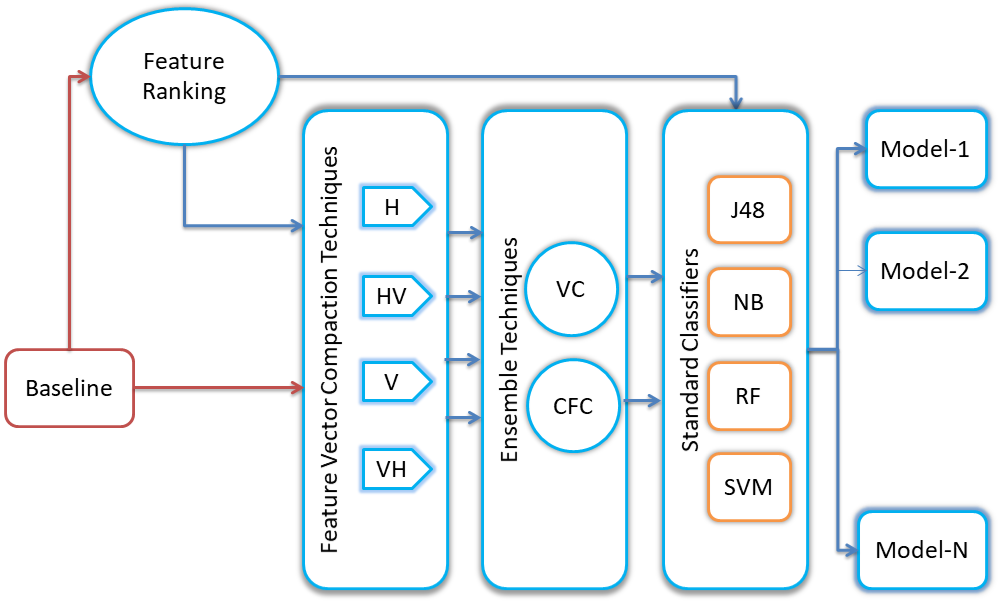
\includegraphics[scale=0.5]{fig/ModelGenOverview.png}
%	\caption{Model Genernation Overview}
%	\label{F:ModelGenOverview}
%\end{figure}

%Additionally, we have constructed the baseline model using all the features, i.e., ignoring the feature ranking exercise; this model is %referred to as Model$_{Base}^{<datasetID>}$. For example, for Adult Binary(F) dataset, for a ranker subset (e.g., R1), for H grouping, for %VC ensemble technique, for J48 classifier the model's name is Model$_\mathrm{i}^\mathrm{AF-R1HVCJ48}$.
